\section{Auswertung}
\label{sec:Auswertung}

\subsection{Statische Methode}
\label{Statische Methode}

\begin{figure}[H]
  \centering
  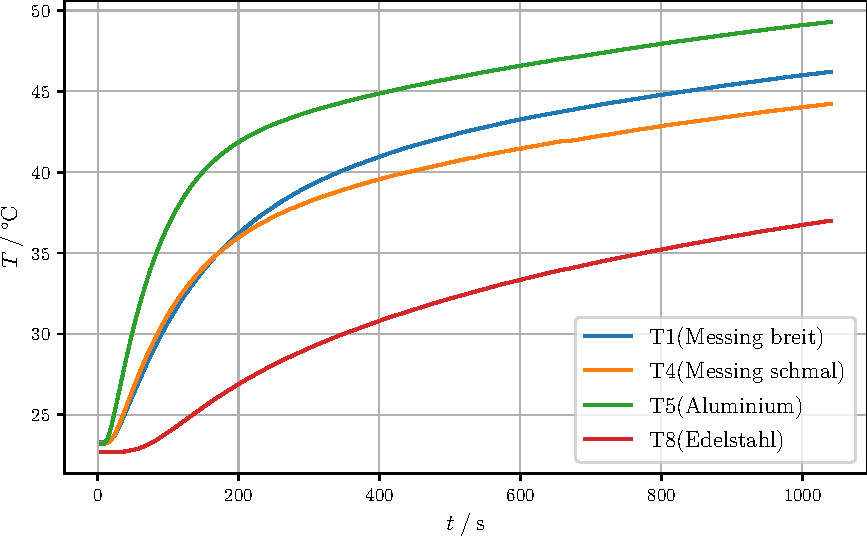
\includegraphics{plot1.pdf}
  \caption{Die Temperaturverläufe der fernen Thermoelemente}
  \label{fig:plot1}
\end{figure}

In Abbildung \ref{fig:plot1} sind die Temperaturverläufe der
weiter vom Peltierelement entfernten Thermoelemente über die Zeit 
dargestellt.\\
Zu erkennen ist der exponentielle Anstieg, der bei allen Stäben zu verschieden Temperaturen 
abflacht. \\
Die Temperatur von Aluminium nimmt am schnellsten zu, die von Edelstahl am langsamsten.\\
Bei den beiden Messingstäben erhitzt zu Beginn der schmale Stab minimal schneller, 
jedoch flacht dessen Kurve früher ab, als die des breiten Stabs, so dass jener eine höhere 
Temperatur erreicht.\\
Nach dem Abflachen der Kurven steigen die Temperaturen aller Stäbe beinahe gleich an.\\
\\
Um zu bestimmen, welcher Stab über die beste Wärmeleitung 
verfügt, werden nun die an den Thermoelementen T1, T4, T5 und T8 nach 700 Sekunden
gemessenen Temperaturen betrachtet und diese in \autoref{tab:TabelleA1} aufgeführt.

\begin{table}[H]
  \centering
  \caption{Die Werte für die fernen Thermoelemente bei $t$ = 700s}
  \begin{tabular}{cccc}
    \toprule
    {$T_{\textrm{Messing, breit}} \mathbin{/} \unit{\degreeCelsius}$} &
    {$T_{\textrm{Messing, schmal}} \mathbin{/} \unit{\degreeCelsius}$} &    % zur not bei einheit $ ... ^\circ$C
    {$T_{\textrm{Aluminium}} \mathbin{/} \unit{\degreeCelsius}$} &
    {$T_{\textrm{Edelstahl}} \mathbin{/} \unit{\degreeCelsius}$} \\
    \midrule
    44,08 & 42,15 & 47,27 & 34,33 \\   
    \bottomrule
  \end{tabular}
  \label{tab:TabelleA1}
\end{table}
\noindent Anhand der \autoref{tab:TabelleA1} lässt sich die Vermutung, dass Aluminium die höchste und 
Edelstahl die geringste Wärmeleitzahl besitzt, stützen. \\
\\
Mit \ref{eqn:WaermeMenge} lässt sich der Wärmestrom $\Phi = \frac{\Delta Q_{21}}{\Delta t}$ zu verschiedenen Zeitpunkten berechnen.
Für den breiten Messingstab ergeben sich der Wärmestrom zu fünf verschieden Zeiten zu den in \autoref{tab:TabelleA2} eingetragenen Werten.\\

\begin{table}[H]   % unfertig ---------
  \centering
  \caption{Der Wärmestrom des breiten Messingstabs zu fünf verschiedenen Zeitpunkten}
  \begin{tabular}{cc}
    \toprule
    {$t \mathbin{/} \unit{\second}$} &
    {$\frac{\Delta Q_{21}}{\Delta t} \mathbin{/} \unit{\watt}$} \\
    \midrule
     100 & -0,6840 \\
     250 & -0,6792 \\
     500 & -0,6770 \\
     750 & -0,6772 \\
    1000 & -0,6772 \\   
    \bottomrule
  \end{tabular}
  \label{tab:TabelleA2}
\end{table}
\noindent Das Vorzeichen des Wärmestroms gibt Auskunft über dessen Richtung.\\


\begin{figure}[H]
  \centering
  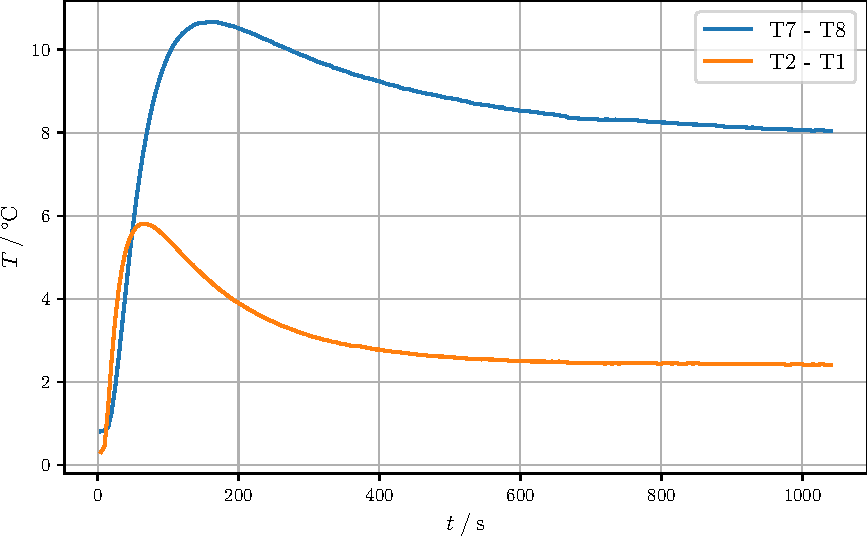
\includegraphics{plot2.pdf}
  \caption{Die Temperaturdifferenzen des Edelstahlstabs ($T_7 - T_8$) und des breiten Messingstabs ($T_2 - T_1$)}
  \label{fig:plot2}
\end{figure}
\noindent In \ref{fig:plot2} ist zu beobachten, dass beide Kurven ähnlich 
steil gegen eine Grenztemperaturdifferenz steigen, die beim Edelstahlstab jedoch deutlich höher
als beim Messingstab liegt.\\ 
Beide Grenztemperaturdifferenzen erreichen in Folge des 
starken Anstiegs ein Maximum, nach jenem sie auf ein Plateau leicht absinken. \\
Das Maximum wird beim Messingstab zeitlich etwas früher erreicht und das Plateau liegt bei 
geringeren Temperaturdifferenzen, als das des Edelstahlstabs.\\


\subsection{Dynamische Methode}
\label{Dynamische Methode}

\begin{figure}
  \centering
  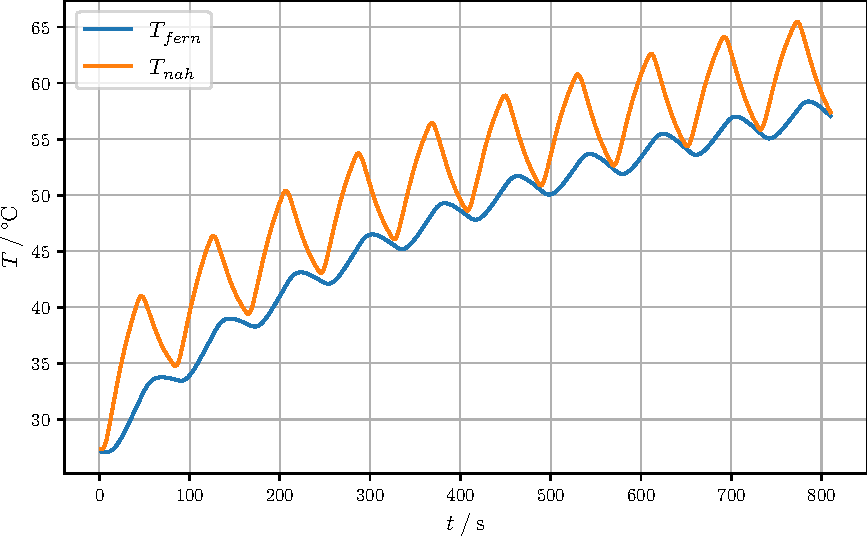
\includegraphics{plot3.pdf}
  \caption{Temperaturverläufe der Thermoelemente T1 und T2 am breiten Messingstab, Periodendauer 80s}
  \label{fig:plot3}
\end{figure}

\begin{figure}
  \centering
  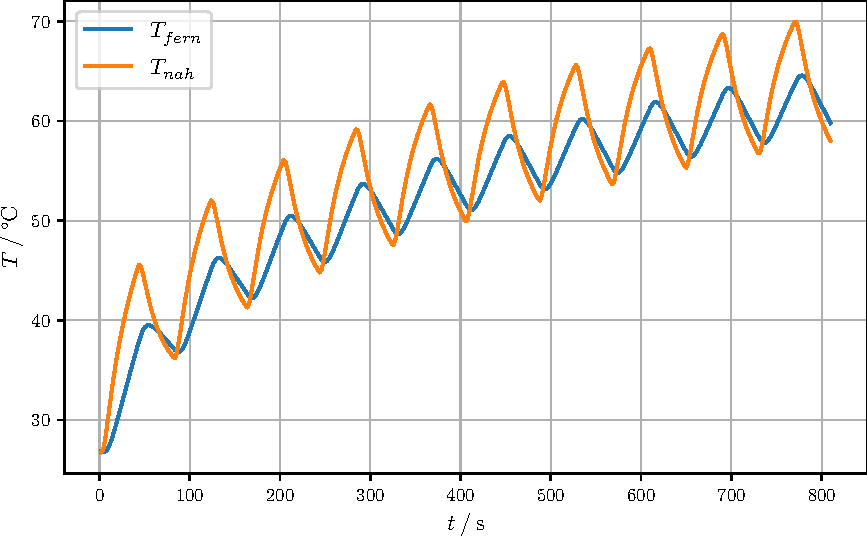
\includegraphics{plot4.pdf}
  \caption{Temperaturverläufe der Thermoelemente am Aluminiumstab, Periodendauer 80s}
  \label{fig:plot4}
\end{figure}

In \autoref{fig:plot3} und \autoref{fig:plot4} sind für den breiten
Messingstab (\autoref{fig:plot3}) und den Aluminiumstab (\autoref{fig:plot4}) die 
Temperaturverläufe der Stäbe bei der Messung nach der Angström-Methode mit einer Periodendauer von 80 Sekunden
über die Zeit aufgetragen.\\



\noindent Es lassen sich die in \autoref{tab:TabelleA3} aufgeführten Werte für den Phasenversatz $\Delta t$ und die Amplituden $A_{nah}$ und $A_{fern}$ ermitteln.

\begin{table}[H]   
  \centering
  \caption{Amplituden und Phasenversatz der Temperaturwelle im breiten Messingstab}
  \begin{tabular}{cccc}
    \toprule
    {$A_{nah} \mathbin{/} \unit{\degreeCelsius}$} &
    {$A_{fern} \mathbin{/} \unit{\degreeCelsius}$} &    % zur not bei einheit $ ... ^\circ$C
    {$\Delta t \mathbin{/} \unit{\second}$} &
    {$\kappa \mathbin{/} \unit{\watt / \meter\kelvin}$} \\
    \midrule
    13,64 & 6,67 & 22 & 88,20 \\   
    11,63 & 5,55 & 18 & 104,25 \\
    10,97 & 4,85 & 18 & 94,49 \\   
    10,69 & 4,41 & 16 & 97,99 \\
    10,41 & 4,09 & 14 & 106,14 \\
    10,28 & 3,90 & 14 & 102,30 \\
     9,93 & 3,62 & 14 & 98,26 \\
     9,96 & 3,57 & 12 & 112,75 \\
     9,78 & 3,39 & 12 & 109,18 \\
     9,61 & 3,30 & 14 & 92,76 \\
    
    \bottomrule
  \end{tabular}
  \label{tab:TabelleA3}
\end{table}
\noindent Für den breiten Messingstab ergibt sich gemittelt
\begin{equation*}
  \kappa = (100.632 \pm 2.434)\unit{\watt\per\meter\per\kelvin}.
\end{equation*}




\noindent Analoges Verfahren wie beim Messingstab ergibt die \autoref{tab:TabelleA4} für Aluminium.

\begin{table}[H]   
  \centering
  \caption{Amplituden und Phasenversatz der Temperaturwelle im Aluminiumstab}
  \begin{tabular}{cccc}
    \toprule
    {$A_{nah} \mathbin{/} \unit{\degreeCelsius}$} &
    {$A_{fern} \mathbin{/} \unit{\degreeCelsius}$} &    % zur not bei einheit $ ... ^\circ$C
    {$\Delta t \mathbin{/} \unit{\second}$} &
    {$\kappa \mathbin{/} \unit{\watt / \meter\kelvin}$} \\
    \midrule
    18,78 & 12,70 & 6 & 419,88 \\
    15,80 &  9,46 & 8 & 243,10 \\
    14,77 &  8,29 & 8 & 215,90 \\   
    14,35 &  7,83 & 8 & 205,84 \\
    14,08 &  7,54 & 8 & 199,66 \\
    13,97 &  7,43 & 6 & 263,33 \\
    13,61 &  7,04 & 6 & 252,217 \\
    13,64 &  7,10 & 6 & 254,65 \\
    13,44 &  6,88 & 8 & 186,22 \\
    13,19 &  6,77 & 6 & 249,28 \\
    
    \bottomrule
  \end{tabular}
  \label{tab:TabelleA4}
\end{table}

\noindent Für den Aluminiumstab ergibt sich gemittelt
\begin{equation*}
  \kappa = (249.0077 \pm 20.7677)\unit{\watt\per\meter\per\kelvin}.
\end{equation*}
